\documentclass{template/socthesis}


\usepackage{subcaption}
%\geometry{showframe}


\graphicspath{ {./images/} }

\addbibresource{sources.bib}

% Title Page
\titlesk{BrailleFeeder - pomôcka pre zrakovo postihnutých}
\school{Stredná odborná škola}
\address{Športová 675, 916 01 Stará Turá}
\author{Juraj Kulich}
\mentor{}
\field{18}
\organizer{Trenčiansky samosprávny kraj}

% Removes „Chapter”
\makeatletter
\def\@makechapterhead#1{%
	% \vspace*{0\p@}%
	{\parindent \z@ \raggedright \normalfont
		\ifnum \c@secnumdepth >\m@ne
		\if@mainmatter
		\Huge\bfseries \thechapter\space%
		%\par\nobreak
		\fi
		\fi
		\interlinepenalty\@M
		\Huge \bfseries #1\par\nobreak
		\vskip 40\p@
}}

\def\@makeschapterhead#1{%
	% \vspace*{50\p@}%
	{\parindent \z@ \raggedright
		\normalfont
		\interlinepenalty\@M
		\Huge \bfseries  #1\par\nobreak
		\vskip 40\p@
}}
\makeatother

% Shows layput in mm
\makeatletter
\renewcommand*{\lay@value}[2]{%
	\strip@pt\dimexpr0.351459\dimexpr\csname#2\endcsname\relax\relax mm%
}
\makeatother

\usepackage{etoolbox}
%\makeatletter
%\patchcmd{\@makechapterhead}{50\p@}{0pt}{}{}
%\patchcmd{\@makeschapterhead}{50\p@}{0pt}{}{}
%\makeatother

\makeatletter
% \patchcmd{<cmd>}{<search>}{<replace>}{<success>}{<failure>}
% --- Patch \chapter
\patchcmd{\@makechapterhead}{50\p@}{\chapheadtopskip}{}{}% Space from top of page to CHAPTER X
\patchcmd{\@makechapterhead}{20\p@}{\chapheadsep}{}{}% Space between CHAPTER X and CHAPTER TITLE
\patchcmd{\@makechapterhead}{40\p@}{\chapheadbelowskip}{}{}% Space between CHAPTER TITLE and text
% --- Patch \chapter*
\patchcmd{\@makeschapterhead}{50\p@}{\chapheadtopskip}{}{}% Space from top of page to CHAPTER TITLE
\patchcmd{\@makeschapterhead}{40\p@}{\chapheadbelowskip}{}{}% SPace between CHAPTER TITLE and text
\makeatother
% Set new lengths
\newlength{\chapheadtopskip}\setlength{\chapheadtopskip}{20pt}
\newlength{\chapheadsep}\setlength{\chapheadsep}{40pt}
\newlength{\chapheadbelowskip}\setlength{\chapheadbelowskip}{15pt}

% TOC settings
\usepackage{tocloft}
\setlength\cftparskip{-10pt}
\setlength\cftbeforesecskip{10pt}
\setlength\cftaftertoctitleskip{15pt}

\begin{document}
	\newgeometry{right=2.5cm}
\maketitle
	\restoregeometry

\newgeometry{left=3.5cm, right=2.5cm, top=2.5cm, bottom=2.5cm}

\makecopyrightstatement{V Starej Turej}
\makethanks{Ďakujem svojmu spolužiakovi Romanovi Mariančíkovi za obetavú pomoc, podmetné  pripomienky a nekonečnú trpezlivosť, ktorú mi počas práce poskytoval.}

\tableofcontents
\thispagestyle{empty}

\chapter*{Zoznam použitých skratiek a symbolov}
\thispagestyle{empty} % Removes page numbering

\begin{adjustbox}{width=1\textwidth}
\begin{tabularx}{\textwidth}{llX }
	\textbf{Skratka} & \textbf{Celý názov} & \textbf{Vysvetlenie} \\
	OS & Operation system & Operačný systém \\
	IoT              & Internet of Things  & Označuje zariadenia	so sieťovou konektivitou umožňujúce vzájomné prepojenie a výmenu dát  \\
	API & Application Programming Interface & Označuje funkcie, triedy, a protokoly knižnice. \\
	HTTP & Hypertext Transfer Protocol & Internetový protokol určený k výmene dát. \\
	PLA & Polylactic Acide & Biologicky rozložiteľný plast používaný pri 3D tlači. \\
	ABS & Acrylonitrile butadiene styrene & Termoplastický kopolymér používaný pri 3D tlači.
	
\end{tabularx}
\end{adjustbox}

\chapter*{Úvod}
\addcontentsline{toc}{chapter}{Úvod}
V roku 2015 malo približne 441 milónov ľudí zrakové postihnutie. Z toho bolo 36 milónov ľudí slepých \cite{bourne2017magnitude}. Takíto ľudia môžu použiť namiesto klasického textu Braillovo písmo, avšak drvivá väčšina pomenovaní a názvov je v klasickom písme. Takisto nikde nenájdeme noviny v Braillovom písme, takže pre slepých je takmer nemožné dostať sa k aktuálnym správam zo sveta.

Momentálne nájdeme taktiež veľmi málo interaktívnych pomôcok pre takýchto znevýhodnených ľudí. Telefóny môžu používať iba pomocou tzv. funkcie čítanie obrazovky, ktorá im číta obsah obrazovky. Táto funkcia je dobrá, ale pre určité úkony môže byť zbytočne zdĺhavá a neintuitívna. Takisto na nej nenájdeme manuálny výstup - braillove písmeno. Ďaľším problémom, s ktorým sa stretávame pri pomôckach pre zrakovo postihnutých sú vysoké ceny. Niektoré displeje na braillovo písmo sa môžu vyšplhať dokonca na tisíce eur. To nás prinúti premýšľať o tom, ako vytvoriť technológiu, ktorá by mohla skutočne zmeniť niečí život.
	
My sa o to snažíme s interaktívnou krabičkou, s relatívne lacne prevedeným braillovým písmenom. Náš systém beží na minipočítači, na ktorom je operačný systém Android Things. Android Things je založený na operačnom systéme Android. Na tomto systéme beží celosvetovo už cez 2 miliardy aktívnych zariadení \cite{ng_2017}. Z toho dôvodu môžeme našu aplikáciu implementovať aj na mobilné zariadenia, na ktoré však nemôžeme pripojiť periférie a tak je funkčnosť obmedzená.
\newpage

%\chapter*{Problematika a prehľad literatúry}
%\addcontentsline{toc}{chapter}{Problematika a prehľad literatúry}
%\newpage

\chapter*{Cieľ a metodika práce}
\addcontentsline{toc}{chapter}{Cieľ a metodika práce}
Cieľom tejto práce je teda prototyp interaktínej krabičky, s ktorou sa budeme snažiť vyriešiť problémy uvedené v úvode. Táto krabička nevidiacim úmožní čítanie článkov z internetu, vypočutie článkov a rozpoznať objekty a text zo snímky vytvorenej fotoaparátom.

Najprv sa budeme snažiť naimplementovať sťahovanie článkov internetu. 
Potom pridáme krabičke hlasový výstup. Po pridaní hlasového výstupu môžeme pridať rozpoznávanie objektov a textu. Potom môžeme dokončiť softvérovú stránku zariadenia pridaním hlasového ovládania a čiastočného slovenského jazyka. Ten sa upltňuje všade okrem hlasového ovládania, ktoré je nastavené na stálu angličtinu. Nakoniec pridáme braillovo elektronické písmo. Všetky komponenty vložíme do našej na mieru vytlačenej krabičky.

Táto práca začína dvoma teoretickými kapitolami. Prvá sa zaoberá vo všeobecnosti Braillovým písmom a druhá približuje základné zásady Android systému. Tretia kapitola popisuje hardvérovú architektúru a funkčnosť zariadenia. Samotnú softvérovú implementáciu opisuje štvrtá kapitola. V poslednej, piatej kapitole, popisujeme postup konštrukcie finálneho produktu. Posledné kapitoly opisujú výsledky testovania a prezentujú celková úspešnosť zariadenia. V závere nájdeme zhodnotené dosiahnuté výsledky a návrhy na možné vylepšenia. 
\newpage

\chapter{Braillovo písmo}
Braillovo písmo je druh písma určeného pre nevidiacich a slabozrakých. Funguje na princípe vyvýšených bodov, ktoré sa dajú čítať hmatom. Zhotovil ho slepý Louis Braille pôvodne z vojenského písma. 

Jedno písmeno Braillovho písma tvorí obdĺžnik bodov s dvoma stĺpcami a troma riadkami, ktorý sa nazýva braillovská bunka. Písmeno Braillovho písma je vo veľkosti rozmeru ukazováka, keďže na brušku ukazováka je najcitlivejší prah hmatu.
Na bunke je možné vytvoriť 64 znakov vrátane prázdnej bunky, ktorá tvorí medzeru. 
Základnú sadu tvoria písmená malej abecedy a interpunkčné znamienka. Čísla a veľké písmená sa tvoria pomocou prefixov.  Napríklad písmeno „c”,  „C” a číslo 3 sa zapíšu tým istým znakom, na rozoznanie sa však používa prefixový znak (Obr. 1.1).

\begin{center}
	\begin{figure}[!ht]
		\centering
		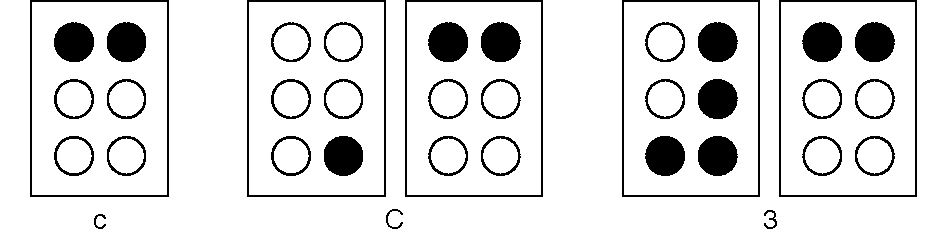
\includegraphics[scale=0.9]{braille}
		\caption{Príklady písmen s ukážkou prefixov}
	\end{figure}
\end{center}

\section{Rôzne normy a formy Braillovho písma}
Najpoužívanejšie formy písma sa nazývajú Grade 1 a Grade 2. Vo forme Grade 1 (plnopis) sa slová prepisujú znak po znaku zatiaľ čo pri forme Grade 2 (skratkopis) dokáže jeden znak znamenať viacero hlások. Skratkopis sa u nás nepoužíva ale je používaný najmä v anglicku.  

\begin{center}
	\begin{figure}[H]
		\centering
		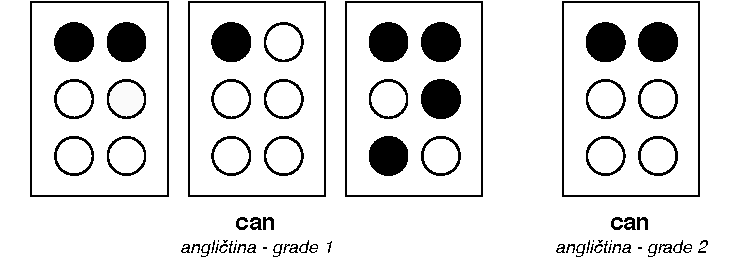
\includegraphics[scale=1]{brailleGrades}
		\caption{Porovnanie anglického slovesa „can” vo forme 1 a 2}
	\end{figure}
\end{center}

Jedným z problémov Braillovho písma je nejednotnosť noriem, ktoré sa výrazne odlišujú. Napríklad medzi českou a slovenskou formou je už v základných písmenách abecedy 7 rozdielov \cite{braille-wiki}. Z dôvodu jednoduchosti a použitia aj slovenského jazyka v ktorom sa skratkopis nepoužíva, v tejto práci používame normu \textit{grade 1}. 

\newpage
\chapter{Android OS}
Android je open source operačný systém pre mobilné zariadenia vyvíjaný spoločnosťou Google. Je postavený na jadre Linuxu. V tejto kapitole si ukážeme vlastnosti  a princípy tohto systému a spôsoby tvorby aplikácii pre tento systém.

\section{Android Things OS}
Android Things je zjednodušená verzia operačného systému Android prispôsobená pre IoT zariadenia. Je navrhnutý tak aby fungoval v inteligentných zariadeniach, napríklad termostatoch alebo kamerách.

\section{Základné princípy Android systému}
V tejto kapitole si priblížime potrebné súčasti pre programovanie pre Android.

\subsection*{Architektúra systému Android}

Architektúra systému Android je rozdelená do niekoľkých vrstiev (Obr. \ref{fig:android_architecture}) pričom každá vrstva využíva služby vrstvy pod ňou. 
\begin{center}
	\begin{figure}[H]
		\centering
		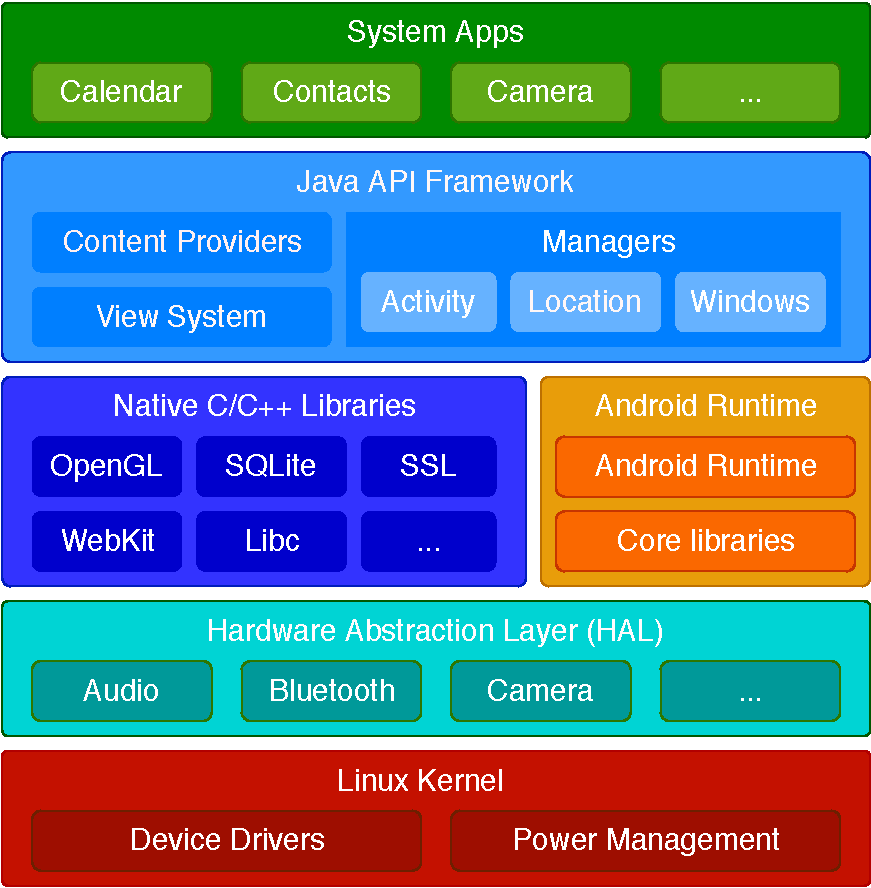
\includegraphics[scale=0.80]{android_architecture}
		\caption{Architektúra systému Android}
		\label{fig:android_architecture}
	\end{figure}
\end{center}

Vrstvy začiatkom od spodnej sú \cite{gandhewar2010google}\cite{androiddevelopers}:
\begin{itemize}
	\item Linux Kernel -- Jadro systému, ktoré poskytuje systémové služby ako sú bezpečnosť, správa pamäte, procesov, sietí a driverov. Slúži taktiež ako abstraktná vrstva medzi hardvérom a softvérom.  
	\item Hardware Abstraction Layer (HAL) -- Hardvérová abstraktná vrstva, ktorá poskytuje štandardné rozhrania vyššej vrstve. Skladá sa z rôznych knižníc, z ktorej kazdá implementuje rozhranie pre špecifický komponent, napríklad kameru alebo Bluetooth.
	\item Libraries -- Obsahuje knižnice písané v jazykoch C a C++. Sú volané cez Java rozhranie. Obsahujú knižnice pre zobrazovanie okien, jadrá pre 2D alebo 3D grafiku, kodeky ako MP3 alebo MPEG-4, SQL databázu alebo WebKit - renderovacie jadro pre prehliadače. 
	\item Android Runtime -- Obsahuje základné knižnice, ktoré poskytujú väčšinu funkcií dostupných v knižniciach jazyka Java. Ďalej obsahuje aplikačný virtuálny stroj Dalvik. 
	
	Virtuálny stroj \textit{Dalvik} -- Vytvára runtime prostredie pre Java aplikácie. Java aplikácie sa najprv prekladajú do bajtkódu pre virtuálny stroj Java, ten sa prekladá do bajtkódu Dalvik a ukladá do súborov .dex - Dalvik Executable a .oed - Optimized Dalvik Executable. Tieto súbory sú menšie a efektívnejšie na Android zariadeniach, ktoré majú slabší procesor a pamäť. Dalvik vytvára pre každú aplikáciu samostatnú inštanciu virtuálneho stroja.  
	 
	\item Java API Framework -- Obsahuje sadu funkcií v jazyku Java potrebných pre tvorbu mobilných aplikácií.
		\begin{itemize} 
		\item View System -- Poskytuje rozhranie pre stavbu užívateľského prostredia
		\item Resource Manager -- Poskytuje prístup k externým zdrojom ako sú reťazce, grafické prvky a súbory s~rozložením prostredia. 
		\item Notification Manager -- Poskytuje prístup k zobrazovaniu notifikáciam v stavovom riadku.
		\item Activity Manager -- Riadi životný cyklus aplikácie.
		\item Content Provider -- Umožňuje zdieľať dáta ostatným aplikáciam.
		\end{itemize}
	\item System Applications -- Je to najvyššia vrstva, ktorá poskytuje množstvo základných aplikácií ako sú email, SMS program, kalendár, aplikácie tretích strán a podobne.
\end{itemize}

\section{Tvorba aplikácií pre Android OS}
\subsection*{Softvérové nástroje}
Pre programovanie pre Android nám stačia nasledovné nástroje:
\begin{itemize}
	\item Java JDK -- Obsahuje základné nástroje na vývoj aplikácií pre Java platformu.
	\item Android SDK -- Poskytuje prístup ku knižniciam Androidu. Obsahuje debugger, Android knižnice, emulátor a dokumentáciu. 
	\item Android Studio -- Oficiálne vývojové prostredie pre Android. 
\end{itemize}

\subsection*{Android Manifest}
Základom každej aplikácie je súbor \textit{AndroidManifest.xml}. Je uložený v koreňovom priečinku každej aplikácie. Tento súbor poskytuje všetky dôležité informácie o aplikácii Android systému. Najdôležitejším je atribút \textit{package}, ktorý označuje unikátny názov aplikácie v Android systéme aj v obchode Google Play. Ďalšie dôležité informácie sú \cite{9781118387108}:
\begin{itemize}
	\item \textbf{Špecifikácie aplikácie} -- Špecifikuje samotné komponenty aplikácie ako sú aktivity \texttt{<activity>}, služby \texttt{<service>}, content providery \texttt{<provider>} a ďalšie. V tagu \texttt{<application>} ďalej nastavujeme meno aplikácie a ikonu aplikácie v Android zariadení. 
	
	V tagu samotnej aktivity nastavujeme meno triedy (parameter \texttt{android:name}), zobrazované meno aktivity (parameter \texttt{android:label}) a často tiež prvok \texttt{<intent-filter>}, ktorý špecifikuje, za akých podmienok sa spustí aktivita.
	
	Príklad špecifikácie aplikácie BrailleApplication, ktorá spustí aktivitu \textit{MainActivity} po spustení aplikácie:
	
	\begin{verbatim}
		<application
		  android:name=".BrailleApplication"
		  android:label="Braille">
		
		  <activity android:name=".ui.main.MainActivity">
		    <intent-filter>
		      <action android:name="android.intent.action.MAIN"/>
		      <category android:name="android.intent.category.LAUNCHER"/>
		    </intent-filter>
		  </activity>
		</application>
	\end{verbatim}
	
	
	\item \textbf{Zoznam povolení} -- Špecifikuje zoznam povolení, ktoré aplikácia potrebuje na fungovanie. Bez potvrdenia povolenia užívateľom nemôže aplikácia použiť danú funkciu. Jedná sa napríklad o prístup k internetu, zápis do pamäte, prístup ku kamere a podobne.
	
	Príklad tagu na povolenie pre používanie internetu: \\
	\texttt{<uses-permission   android:name="android.permission.INTERNET" />
	}
	\item \textbf{Minimálna verzia systému} -- Určuje minimálnu verziu Android systému, potrebnú na správne fungovanie aplikácie. Verzie sa od seba môžu odlišovať novými triedami, metódami alebo parametrami. 
	
	Príklad tagu na nastavenie minimálnej verzie systému na verziu 25 (Android 7.1.1): \\
	\texttt{<uses-sdk android:minSdkVersion="25" />}	
\end{itemize}

\subsection*{Lokalizácia aplikácie}
Android funguje na zariadeniach v mnohých regiónoch. Aby sme nemuseli vyvíjať viac aplikácií s rôznymi jazykmi používame lokalizáciu. Lokalizácia sa stará o prispôsobenie textu, obrázkov, čísel alebo meny podľa regiónu použitia. 

Android na takéto zmeny používa prepínanie zdrojov. Zdroje môžu obsahovať rôzne nastavenia pre rôzne prípady ako napr. rozloženie prostredia pre zvislú polohu a horizontálnu polohu telefónu, rozdielne obrázky pre rôzne rozlíšenia, lokalizované reťazce pre rôzne jazyky, atď.

Základné zdroje nájdeme v zložke \texttt{/res/values}. V tejto zložke je automaticky vytvorený súbor \texttt{strings.xml}, ktorý obsahuje reťazce používané v prápade že nie je dostupná žiadna iná lokalizácia. Po pridaní slovenskej lokalizácie sa vytvorí nová zložka \texttt{/res/values-sk-rSK/strings.xml}. Akonáhle bude mať zariadenie nastavené slovenský jazyk, aplikácie bude používať zdroje zo slovenskej lokalizácie. V aplikácii tak nie je vhodné používať konštatné reťazce ale reťazce zo zdrojov. V našom prípade používame slovenskú lokalizáciu pre zvukový výstup zariadenia.

\subsection*{Ukladanie dát}
Android poskytuje niekoľko možností na ukladanie dát. Tieto možnosti sa rozlišujú podľa toho o aký typ dát ide, podľa veľkosti dát alebo podľa možnosti prístupu. Tieto možnosti sú\cite{persistence}:
\begin{itemize}
	\item \textbf{Interná pamäť zariadenia} -- Dáta sú ukladané v internej pamäti zariadenia.
	\item \textbf{Externá pamäť zariadenia} -- Dáta sú ukladané v externej pamäti zariadenia, napríklad na SD kartu.
	\item \textbf{Databáza} -- Databázy sú využívané na ukladanie štrukturovaných dát. Dáta sú ukladané v SQL databáze. My tento typ používame pri ukladaní článkov.
	\item \textbf{Shared preferences} -- Dáta sú ukladané v množinách dvojíc kľúč–hodnota. Ukladáme s nimi primitívne typy dát ako sú int, float, atď. My ich využívame pri ukladaní súčasnej lokalizácie.
\end{itemize}

\subsection*{Procesy a vlákna}
Predvolene bežia všetky komponenty aplikácie v jednom procese a vlákne (tzv. hlavné vlákno). V niektorých prípadoch je dôležité vykonávať niektoré metódy v iných procesoch a vláknach, aby sme neblokovali chod hlavného vlákna. Ak v hlavnom vlákne vykonávame dlhotrvajúce operácie ako sú pristupovanie k databáze alebo k internetu, aplikácia môže spadnúť. V našej aplikácií používame rozdielne vlákna napríklad pri fotografovaní, sťahovaní článkov alebo k prístupu k databáze.

\subsection*{Práca s perifériami}
Pre prácu s perifériami slúži systémová služba \textit{PeripheralManager}. Pomocou tejto triedy dokážeme nastavovať a ovládať  GPIO piny. Taktiež obsahuje callback na prijímanie signálov z pinov.
\newpage

\chapter{Hardvérová architektúra zariadenia}
V tejto kapitole si ukážeme architektúru nášho zariadenia. Ukážeme si časti z ktorých sa skladá a ako prispievajú k správnej funkčnosti.

\begin{center}
	\begin{figure}[h]
		\centering
		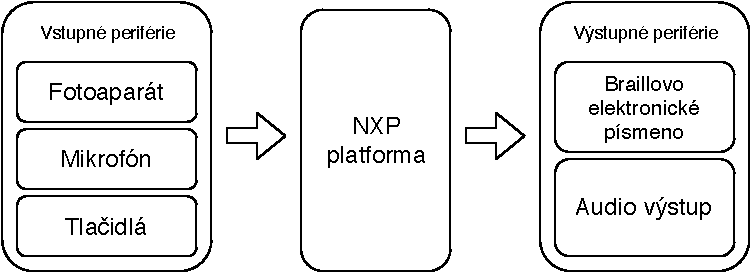
\includegraphics{brailleblock}
		\caption{Bloková schéma zariadenia}
	\end{figure}
\end{center}

\section{Vývojová doska}
Mozog zariadenia tvorí HW platforma NXP i.MX7D. Táto platforma obsahuje množstvo zberníc a pinov na pripojenie rôznych zariadení. Tu využívame USB na pripojenie mikrofónu, RJ45/Wi-Fi na pripojenie k internetu, konektor na pripojenie fotoaparátu, 3.5mm jack na pripojenie audio zariadení a univerzálne piny GPIO na pripojenie ostatných potrebných periférií(tlačidlá, cievky, …).
Táto platforma má procesor ARM Cortex-A7 - 1GHz, 512MB pamäte RAM a 4GB internú pamäť. Fotoaparát sa pripája pomocou MIPI CSI rozhrania. Operačný systém tejto platformy je Android Things.

\section{Časti elektroniky}
\subsubsection{Elektronické Braillovo písmeno}
Základným prvkom tejto vlastne vyrobenej periférie je 6 elektronicky ovládaných solenoidov usporiadaných do obdĺžnika - tvoria jedno Braillovo písmeno. V platforme sa články prekonvertujú do kombinácii núl a jednotiek, ktoré sa odosielajú na vstupy tohto zariadenia pomocou GPIO pinov, a podľa toho vytvoria vysúvaním dané písmeno. 

Solenoid je súčiastka, ktorej kovová časť sa za pomoci magnetu a cievky dokáže vysúvať a zasúvať. Keďže naša platforma dokáže na jednom GPIO pine poskytnúť maximálny prúd okolo 20mA, napájanie je riešené pomocou externej batérie. Tým pádom potrebujeme 6 optočlenov a tranzistorov na zopínanie cievok. Pri dodaní signálu sa cievka kovová časť cievky zasunie.

\subsubsection{Batérie}
Slúžia na napájanie dosky a modulu s cievkami(Braillovo písmeno). Používame tri nabíjateľné 3400mAh 3.7V batérie typu 18650. Na napájanie dosky používame napäťový booster z 3.7V na 5V.

\subsubsection{GPIO piny}
General-purpose input/output - sú digitálne piny, ktoré dokážu slúžiť aj ako vstupy aj výstupy podľa potreby. Používame ich ako výstupy pre posielanie impulzov do cievok a ako vstupy pri tlačidlách. 

\subsubsection{USB vstup}
Slúži na pripojenie USB mikrofónu.

\subsubsection{3.5mm jack}
Slúži na pripojenie audio zariadení pre hlasový výstup.

\section{Režimy použitia}
Naše zariadenie dokáže pracovať	 vo viacerých režimoch:
\begin{enumerate}
\item Prehrávanie článkov na Braillovom písmene -- článok sa rozdelí na písmená a každé písmeno sa skovertuje na príslušný kód, podľa ktorého sa zobrazí výstupe.
\item Prehrávanie článkov cez reproduktor.
\item Vstup pre základné úkony pomocou tlačidiel. 
\begin{itemize}
\item prepínanie článkov
\item nastavenie hlasitosti
\item nastavenie rýchlosti prepínania Braillovho písma.
\end{itemize}
\item Vstup pre rozšírené úkony cez mikrofón (hlasové ovládanie) -- hlasové ovládanie je z dôvodu gramatickej nestálosti slovenského jazyka dostupné iba v anglickom jazyku.
\begin{itemize}
\item prepínanie článkov dopredu/dozadu
\item nastavenie hlasitosti na presnú hodnotu
\item určenie kategórie vyhľadávaných článkov 
\item vyhľadávanie článkov o konkrétnej téme
\item uloženie článkov do offline pamäte
\item načítanie uložených článkov
\item vytvorenie snímku
\item zmena jazyka prostredia do slovenského jazyka
\item pomocný príkaz pre nápovedu
\end{itemize}
\end{enumerate}

\chapter{Softvérová architektúra zariadenia}
Táto kapitola popisuje softvérovú časť zariadenia, použité technológie a zámery.

\section*{Práca s fotoaparátom}
Na ovládanie fotoaparátu potrebujeme pridať oprávnenie do manifestu, viď. 2.3.  Pomocou triedy \texttt{CameraDevice} dokážeme fotoaparát nastaviť a vytvárať snímky. Hlavnou výhodou tejto metódy prístupu k fotoaparátu, je integrácia fotoaparátu priamo do aplikácie. Úkon fotografovania je tak riadený stiskom tlačítiek, ktoré si sami zadefinujeme. Vytvorená fotografia je ďalej v aplikácii reprezentovaná ako pole bitov, s ktorým môžeme ďalej pracovať. V našej práci sú všetky úkony s fotoaparátom v triede \texttt{CameraService}.

\section*{Práca s audiom}
Na nahrávania audia potebujeme taktiež oprávanenie v manifeste.  Pomocou triedy \texttt{AudioRecord} dokážeme zaznamenávať zvuk a nastavovať atribúty nahratého zvuku ako sú \cite{audio}: \\
\begin{itemize}
	\item \textbf{Zdroj audia} -- Nastavuje zdroj zvukových nahrávok. V našom prípade to je mikrofón na USB vstupe.
	\item \textbf{Vzorkovacia frekvencia} -- Zvuk je analógový signál. Aby sme ho mohli dátovo reprezentovať, zadefinujeme počet vzorkov prenášaných za jednotku času v každom momente. Náš mikrofón podporuje 16 kHz, t.j. 16000 vzoriek za sekundu.
	\item \textbf{Formát audia} -- Definuje formát, v ktorom je uložený zvuk. Môže byť stratový  alebo bezstratový. My používame bezstratový raw formát PCM.
	\item \textbf{Kanál} -- Je to reprezentácia zvuku, ktorý ide z alebo do jedného zvuku. 
\end{itemize}

Pretože niektoré metódy boli vysoko nad našou úrovňou vedomostí, naše triedy \texttt{SpeechRecorder.java} a \texttt{SpeechToText.java} sú rozšírením už existujúcich Java tried získaných z ukážky\cite{code-audio} na používanie Speech-To-Text API.

\subsection*{Konverzia textu na braillový výstup}
Na to aby sme dokázali text zobraziť na našej braillovej bunke, potrebujeme preložiť text na digitálny výstup. Ako vieme z hardvérovej časti, po dodaní signálu do cievky sa jej kovová časť zasunie. To znamená, že v základnom stave musíme mať na všetkých stupoch privedený signál 1. Na reprezentáciu písmen, čísel a znakov používame skupiny jednotiek a núl. Tieto skupiny máme zadefinované v triede \texttt{Braille.java}. Každá skupina obsahuje 6 hodnôt, z ktorej každá hodnota odkazuje na jeden bod v braillovom písme. 

Samotný text prekladáme v triede \texttt{BrailleConverter.java}. V tejto triede prechádzame cez text a nájdené písmená prekladáme na braillové písmená. Po preložení všetkých slov vrátime digitálny výstup a pošleme na piny.	

\subsection*{Hlasové ovládanie}
Táto časť obsahuje detaily o hlasovom ovládaní. Všetky príkazy nájdeme v prílohe \textit{A. Dostupné príkazy na hlasové ovládanie}.

\subsubsection{Kategórie}
Dostupné kategórie pri vyhľadávaní článkov sú:
\begin{itemize}
	\item biznis (príkaz \textit{business})
	\item zábava (príkaz \textit{entertainment})
	\item zdravie (príkaz \textit{health})
	\item veda (príkaz \textit{science})
	\item šport (príkaz \textit{sport})
	\item technológie (príkaz \textit{technology}) 
\end{itemize}

\subsubsection{Jazyk prostredia}
Pod jazykom prostredia rozumieme jazyk vyhľadávaných článkov, nárečie hovoreného výstupu a jazyk hovoreného výstupu. Hlasové ovládanie je iba v angličtine. Prostredie meníme pomocu zmeny lokalizácie.

\subsubsection{Príkaz \textit{about}}
Príkazom \textit{about} definujeme o čom sa majú články vyhľadávať. Napríklad príkaz na vyhľadávanie článkov o mačkách bude: about cats. Takýmto spôsobom dokážeme vyhľadávať články o veciach, ľudoch, štátoch, atď.

\subsubsection{Hlasitosť}
Hlasitosť nastavujeme presne na percentá alebo po 12.5\% maximálnej hlasitosti zariadenia. Príkaz na nastavenia hlasitosti na polovicu bude teda: set volume to 50\%.

\section{Použité technológie}
Na vývoj hlavného programu bol použitý jazyk Java z dôvodu predchádzajúcich skúseností s týmto jazykom a veľmi rozšírenou komunitou. Pri programovaní sme sa snažili dodržať všetky koncepty objektovo-orientovaného programovania ako sú dedičnosť, abstrakcia, zapuzdrenosť a polymorfizmus. \\

Použili sme oficiálne vývojové prostredie od Googlu - Android Studio. Toto prostredie je postavené na vývojovom prostredí IntelliJ IDEA a podporuje dopĺňanie príkazov, refaktoring alebo analýzu kódu. Toto prostredie obsahuje aj emulátor, ktorý slúži ako virtuálne Android zariadenie. Na ukladanie údajov používame SQL databázu.

\subsection*{Protocol Buffers}
Protocol Buffers je binárny formát používaný na výmenu dát. Pomocou tohto formátu dokážeme zadefinovať štruktúru triedy a vytvoriť tzv. schému. Z tejto schémy sa dá potom vygenerovať trieda pre konkrétny, takmer akýkoľvek, jazyk. Tieto Protocol Buffers používa aj Google pre svoje knižnice. V zložke \texttt{.../main/proto/google} nájdeme všetky \texttt{.proto} súbory od Googlu, ktoré používame na prístup k niektorým knižniciam.


\subsection*{Použité knižnice}
\subsubsection{Butterknife}
Knižnica Butterknife generuje k prvkom z rozhrania(napr. tlačidlo) štandardizovaný kód, čím nám skracuje dĺžku kódu a robí ho prehľadnejším.
\subsubsection{OkHttp}
Knižnica OkHttp slúži na posielanie a prijímanie HTTP a HTTP/2 požiadavok a prijímanie/spracovávanie odpovedí zo servera.
\subsubsection{Retrofit}
Retrofit je REST (Representational State Transfer) klient s typovou kontrolou. REST je rozhranie, ktoré definuje metódy pre prístup k dátam - vytvoriť, zmazať, upraviť, získať. Pomocou neho získavame dáta z internetu a ukladáme do našich Java tried.
\subsubsection{Room}
Poskytuje abstraktnú vrstvu nad SQL databázou, umožňuje lepší prístup k databáze použitím menšieho množstva kódu a overuje dotazy na databázu.
\subsubsection{Cloud Vision API}
Umožnuje zistiť obsah z fotografie. Detekuje skupiny objektov a vecí (napr. rastliny, zvieratá, …) a extrahuje tlačený text.
\subsubsection{Cloud Speech-To-Text API}
Konvertuje audio do textu. Slúži na hlasové ovládanie.
\subsubsection{Cloud Translation API}
Poskytuje rozhranie na preklad textu. V našom prípade z angličtiny do slovenčiny. Toto API zatiaľ nepodporuje Android a preto posielame požiadavku na server s textom, ktorý chceme preložiť.

\chapter{Konštrukčná časť}
Naše zariadenie obsahuje veľa komponentov, ktoré musia byť dostupné z vonkajšej časti zariadenia. Jedná sa napríklad o cievky, koncovku RJ-45 alebo mikrofón. Z toho sme usúdili, že najlepšie bude, ak naše komponenty umiestnime do plastovej krabičky. Kedže sme potrebovali veľmi atypické rozmery okolo 20x15x4cm, bol veľký problém zohnať takú nízku krabičku. Preto sme sa rozhodli, že si ju vytlačíme na 3D tlačiarni. 

\section{3D tlač}
Trojrozmerná tlač je technológia, ktorá vytvára reálny trojdimenzionálny objekt pomocou nanášania vrstiev. Takýmto spôsobom dokážeme vytvoriť produkty z plastového materiálu. 3D tlačiarne tlačia na základe digitálnych dát, ktoré im poskytneme.

\subsubsection{PLA plast}
Naša krabička je vyrobená z PLA plastu. Tento plast je vyrobený z obnoviteľných zdrojov ako sú zemiaky a kukurica. Jeho výhodou je teda biologická rozložiteľnosť. Takýto plast sa dokáže rozložiť o stovky až tisíce rokov skôr, ako z ropy vyrobený plast ABS. Napriek tomu majú však tieto plasty podobné vlastnosti. Výrobou tohto plastu tak neškodíme životnému prostrediu.

\subsubsection{Softvér Fusion 360}
Na vytvorenie podkladov pre 3D tlačiareň sme využili softvér Fusion 360. Tento softvér slúži na vytváranie 3D modelov. Na ukážku prostredia a nášho vytvoreného modelu odkazuje príloha. 

\newpage

\chapter*{Výsledky práce}
\addcontentsline{toc}{chapter}{Výsledky práce}
V tejto kapitole zhodnotíme úspešnosť rozpoznávania objektov a textu z fotografie. Na testovanie boli použité hlavne fotografie vytvorené v domácom prostredí. Neskôr výsledky zhodnotíme.

\section{Príklady zhotovených snímkov a výsledkov spracovania}


\begin{figure}[htp]	
	\captionof{table}{Výsledky spracovania obrazu pre objekty}
	\begin{tabularx}{\textwidth}{|l|X| }
		\hline
		\textbf{Snímok} & \textbf{Výsledky spracovania} \\
		\hline
		a) & technology(technické vybavenie), electronic device(elektronické zariadenie), remote control(diaľkový ovládač), plant(rastlina), illustration(ilustrácia) \\
		\hline
		b) & green(zelená), technology(technické vybavenie), electronic device(elektronické zariadenie), laptop, architecture(architektúra) \\
		\hline
		c) & water(voda), product(bottle), plastic bottle(plastová fľaša), water bottle(fľaša na vodu) + text(Pepsi) \\
		\hline
		d) & green(zelená), musical instrument(muzikálny inštrument), musical instrument accessory(príslušenstvo muzikálneho inštrumentu), string instrument accessory(príslušenstvo strunového nástroja) \\
		\hline
		e) & apple(jablko), food(jedlo), plant(rastlina), fruit(ovocie), 
		vegetarian food(vegetariánske jedlo) \\
		\hline
	\end{tabularx}
\end{figure}

Z výsledkov spracovania obrazu pre zisťovanie objektov na snímku môžeme vidieť relatívnu presnosť. Častokrát sa však stáva že sú objekty označené vo všeobecnosti. Ďaľšou vecou, ktorú si môžeme všimnút je, že sa vo výsledkoch často objavuje objekt green. To je spôsobené nekvalitnou kamerou, ktorá v horších svetelných podmienkach zafarbuje fotografiu na zeleno.

\begin{figure}[H]	
	\captionof{table}{Výsledky spracovania obrazu pre text}
	\begin{tabularx}{\textwidth}{|l|X| }
		\hline
		\textbf{Snímok} & \textbf{Nájdený text} \\
		\hline
		a) & DIGITAL MULTIMETER, K200, Logitech \\
		\hline
		b) & STORCK, Toffifee, Caramel with Creamy Nougat and Choco \\
		\hline
		c) & A RELUCTANT EXERCISER CHANGES HIS MIND, antonioa fifty four year old on of wo succesful Italian restaurants wss in my class on doctor's orders. He had high blood pressure and cholesterol and his waist size crept up an inch every year. If he didn't change his lifestyle, his doctor warned him he was going to collapse of a heart attack... \\
		\hline
	\end{tabularx}
\end{figure}

Z výsledkov spracovania obrazu pre zisťovanie text na snímku môžeme vidieť taktiež relatívnu presnosť. Ako vidíme, takýmto spôsobom môžeme spracovávaž aj text, ktorý je napísaný rôznymi typmi alebo veľkosťami písma.

\section*{Podmienky pre presnejšie spracovanie}
V tejto časti si ukážeme rôzne podmienky, od ktorých závisí výsledná kvalita spracovania. Situácie ovplyvňujúce tieto podmienky môžu vzniknúť či už kvôli hardvéru, alebo nevyhovujúcemu okoliu.

\subsubsection*{Natočenie kamery voči snímanému objektu}
Natočenie kamery zohráva jednu z najdôležitejších úloh pri spracovaní fotografie. Výhodou nášho zariadenia je že aj pri nesprávnom natočení dokáže rozoznávať objekty. Avšak text môže byť pri zlom natočení nepresnejší. 

\subsubsection*{Svetelné podmienky}
Svetelné podmienky taktiež ovplyvňujú výsledok spracovania. Ako sme mohli vidieť v sekcii 2.1, zariadenie pri zlých svetelných podmienkach sfarbuje snímky do zelenej farby a tak robí spracovanie nepresným. 

\subsubsection*{Rozostrenie snímaného objektu}
Rozostrenie objektov môže spôsobiť splývanie hrán, podľa ktorých sa zisťujú objekty na fotografii. Keďže náš fotoaparát neobsahuje zaostrovanie a stabilizátor, môže sa stať oveľa častejšie že fotografie budú neostré a výsledky nepresné.

\subsubsection*{Vzdialenosť od snímaného objektu}
Pri väčšej vzdialenosti od zachytávaného objektu môžu vzniknúť nepresnosti kvôli širokému záberu. Na fotografii sa tak môžu nachádzať ďalšie objekty alebo text, ktoré budú ovplyvňovať výsledok spracovania. 

\mbox{}\\
Nemyslíme si, že je v tomto prípade dôležité spracovávať percentnú úspešnosť a spracovávať štatistiky.


\newpage
\chapter*{Záver}
\addcontentsline{toc}{chapter}{Záver}
Na začiatku práce bolo pre nás dôležité preštudovať Braillovo písmo. Potom sme implementovali všetky potrebné funkcie, pridali a vytvorili sme potrebné periférie a zariadenie sme vložili do vhodnej krabičky. Nakoniec sme vykonali testovanie naších periférií - hlasové rozpoznávanie a rozpoznávanie objektov a textu.
 
Hlavným prínosom tejto práce je teda možnosť umožniť ľudom so zrakovými poruchami

Naše zariadenie sme sa snažili čo najviac navrhnúť tak, aby bolo pre ľudí so zrakovými vadami čo najintuitívnejšie. Kládli sme dôraz na to, aby museli užívatelia k vykonaniu všetkých potrebných úkonov urobiť čo najmenší počet krokov. Pre reálne použitie medzi slepými je ešte potrebné naše zariadenie testovať priamo medzi týmito ľudmi a zapracovať ich poznatky. 

Pri návrhu zariadenia nás napadlo viacero možností ako by sa dalo zariadenie upraviť alebo vylepšiť. Myslíme, že naše zariadenie by mohlo mať vysoký potenciál nie len ako pomôcka poskytujúca novinové články a rozpoznávanie obrazu a textu, ale aj ako edukačná pomôcka. 
Ak by sme prišli na spôsob ako importovať elektronické knihy do zariadenia, naše zariadenie by mohlo slúžiť ako elektronická čítačka kníh pre zrakovo postihnutých. Ďaľej by sa dalo zariadenie využiť iba ako elektronické braillovo písmeno s Bluetooth pripojením k telefónu. Takýmto pripojením by bolo teoreticky možné na našom zariadení zobraziť akýkoľvek obsah z telefónu. 
Momentálnou nevýhodou zariadenia je jeho veľkosť. Toto je však spôsobené použitím celej prototypovacej jednotky NXP Pico. Ak by sme použili iba potrebné komponenty a periférie zariadenia, naše zariadenie by bolo možné zmenšiť aj o tretinu. Takisto dokážeme zmenšiť naše Braillovo písmeno použitím malých SMD súčiastok.

\newpage
\chapter*{Zhrnutie}
\addcontentsline{toc}{chapter}{Zhrnutie}
\newpage

\printbibliography[title=Zoznam použitej literatúry]
\addcontentsline{toc}{chapter}{Zoznam použitej literatúry}
\newpage
\pagenumbering{gobble}

\chapter*{Zoznam príloh}
\addcontentsline{toc}{chapter}{Zoznam príloh}
\newpage

\begin{appendices}
	
	\chapter{Zdrojový kód}
	%Zdrojový kód nájdeme na úložisku GitHub: \url{github.com/yuro8/BrailleFeeder}.
	V tejto časti si ukážeme niektoré ukážky z nášho zdrojového kódu.
	Zdrojový kód je z praktických dôvodov okomentovaný po anglicky.
	
	\section*{Štruktúra zdrojového kódu}
	Balíčky v našom zdrojovom kóde:
	\begin{itemize}
		\item /data --
		\item /remote
		\item /brailleutils
		\item /apis
	\end{itemize}

	\chapter{Abeceda}
	
	\chapter{Dostupné príkazy na hlasové ovládanie}
	\begin{figure}[htp]	
	\captionof{table}{Príkazy dostupné pri hlasovom ovládaní}
	\begin{tabularx}{\textwidth}{|l|X| }
		\hline
		\textbf{Príkaz} & \textbf{Úkon} \\
		\hline
		help & Povie všetky dostupné príkazy aj s príkladmi \\
		\hline
		switch to slovak/english & Zmení prostredie do daného jazyka. \\
		\hline
		next article & Prepne výstup na nasledujúci článok. \\
		\hline
		previous article & Prepne výstup na predošlý článok. \\
		\hline
		category \textit{kategória} & Vyhľadá články v kategórií \textit{x} \\
		\hline
		about \textit{x} & Vyhľadaná články o slove \textit{x}. \\
		\hline
		take photo & Vytvorí snímok fotoaparátom. \\
		\hline
		save article & Uloží článok do offline pamäte. \\
		\hline
		show/load saved articles & Načíta všetky články z offline pamäte. \\
		\hline
		set volume to \textit{x} percent & Nastaví hlasitosť na \textit{x} percent. \\
		\hline
		volume up & Zväčší hlasitosť o 12.50\%. Po zvýšení nad 100\% sa cyklus opakuje od 0\%. \\
		\hline
	\end{tabularx}
	\end{figure}


	\chapter{Časti elektroniky a schémy zariadenia}
	
	\begin{center}
		\begin{figure}[h]
			\centering
			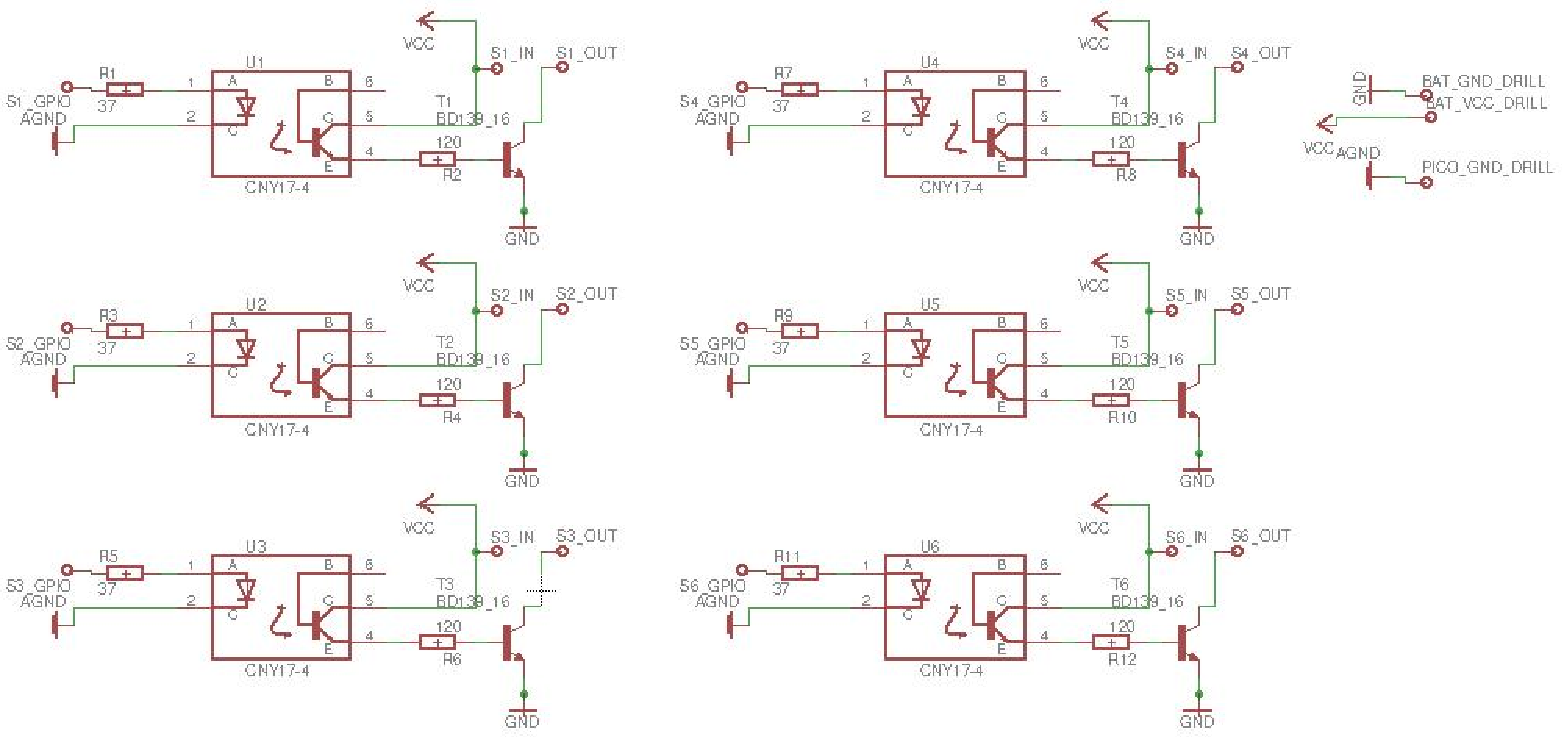
\includegraphics[width=\textwidth,height=\textheight,keepaspectratio]{scheme}
			\caption{Schéma nášho braillovho elektronického písmena}
		\end{figure}
	\end{center}

	\begin{center}
		\begin{figure}[h]
			\centering
			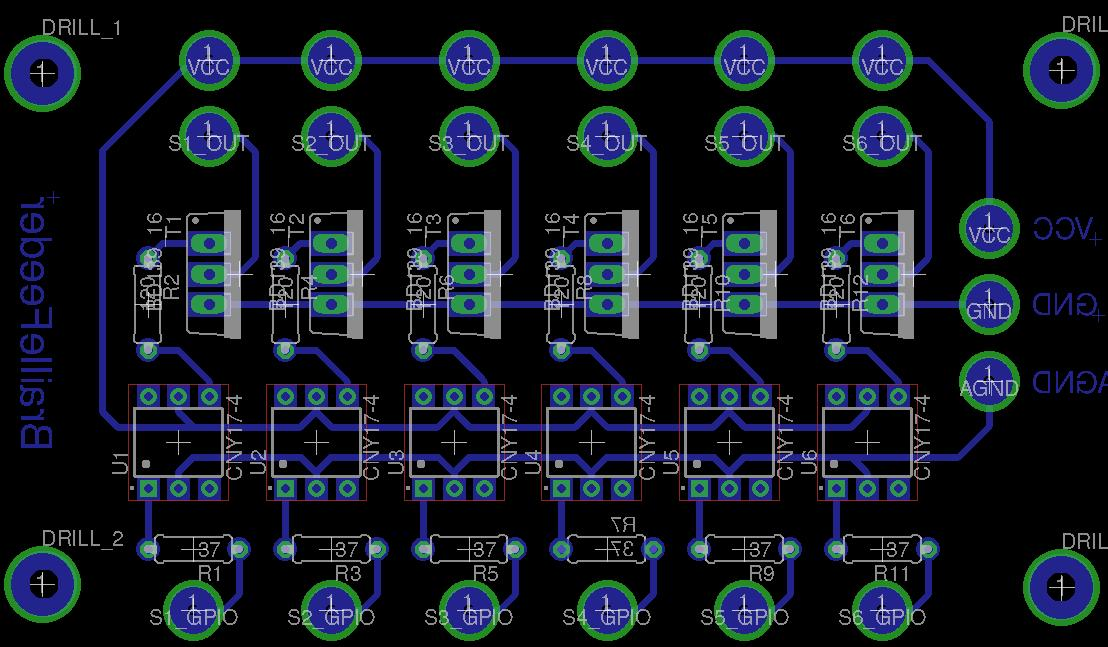
\includegraphics[width=\textwidth,height=\textheight,keepaspectratio]{board}
			\caption{Návrh nášho braillovho elektronického písmena}
		\end{figure}
	\end{center}

	\chapter{Užívateľské prostredia a 3D návrh}
	

\end{appendices}
 
%\layout
\end{document}          
